\section{Determination of $\rho$}
\label{sec:rho}

The value of the $\rho$ parameter can be extracted from the differential cross-section thanks to Coulomb-nuclear interference. Section \ref{sec:rho cni} summarises our modelling of this effect and Section \ref{sec:rho anal} describes data fits and results.

%----------------------------------------------------------------------------------------------------
\subsection{Coulomb-Nuclear Interference}
\label{sec:rho cni}

\TODO{some introduction} More complete description is available in \cite{totem-8tev-1km}, Section 6.

The Coulomb amplitude can be derived from QED. In one-photon approximation it yields cross-section
\begin{equation}
\label{eq:coul cs}
	{\d\sigma^{\rm C}\over \d t} = {4\pi\alpha^2\over t^2}\,{\mathcal{F}}^4\ ,
\end{equation}
where $\alpha$ is the fine-structure constant and $\mathcal{F}$ represents an experimentally determined form factor -- we have used the one from Ref.~\cite{puckett10}.

At low $|t|$, the modulus of the nuclear amplitude is modelled as
\begin{equation}
\label{eq:nuc mod}
\left | {\cal A}^{\rm N}(t) \right | = \sqrt{s\over\pi} {p\over \hbar c} \sqrt{a} \exp\left( {1\over 2} \sum\limits_{n = 1}^{N_b} b_n\, t^n \right)\ ,
\end{equation}
in agreement with the experimental observation. The $b_1$ parameter is responsible for the leading exponential decrease, other $b_n$ parameters can describe small deviations from the leading behaviour. Since the calculation of CNI may, in principle, involve integrations (e.g.~Eq.~(\ref{eq:int kl})), it is necessary to extend the nuclear amplitude meaningfully to higher $|t|$ values, too. At that region, the amplitude is fixed to a form that describes well the dip-bump structure observed in the data, see e.g.~Figure~\ref{fig:fit exp3 0.15}, right. In order to avoid numerical problems, the intermediate $|t|$ region is modelled with a continuous and smooth interpolation between the low and high-$|t|$ parts. \TODO{check this: It will be shown that altering the extended part of the nuclear amplitude ($|t| > 0.2\un{GeV^2}$) within reasonable limits has negligible impact on the results presented later on.}

Several parametrisations have been considered for the phase of the nuclear amplitude. Since one of the main goals of this analysis is to compare the newly obtained $\rho$ value with those at lower energies, we have focused parametrisations similar to the past analyses. Consequently we have considered phases with slow variation at low $|t|$: constant, Bailly and standard from \cite{totem-8tev-1km}. No dependence of the results on this choice was observed and therefore only the constant phase
\begin{equation}
\label{eq:nuc phase con}
\arg {\cal A}^{\rm N}(t) = {\pi\over 2} - \arctan\rho = \hbox{const} \ .
\end{equation}
will be retained in what follows. 

We have used the most general interference formula available so far \cite{kl94}:
\begin{equation}
\label{eq:int kl}
	\begin{aligned}
		{\d\sigma\over \d t}^{\rm C+N} =& {\pi (\hbar c)^2 \over s p^2} \left | {\alpha s\over t} {\cal F}^2
			+ {\cal A}^{\rm N}\, \Big[1 - \I\alpha G(t)\Big] \right |^2\ ,\cr
		G(t) =& \int\limits_{-4p^2}^0 \d t'\, \log {t'\over t} {\d\phantom{t'}\over \d t'} {\cal F}^2(t')\cr
			  &- \int\limits_{-4p^2}^0 \d t' \left( {{\cal A}^{\rm N}(t') \over {\cal A}^{\rm N}(t)} - 1 \right) { I(t, t')\over 2\pi }\ , \cr
		I(t, t') =& \int_0^{2\pi} \d\phi\ {{\cal F}^2(t'')\over t''}\ ,\cr
		t'' =& t + t' + 2\sqrt{t\, t'} \cos\phi\ .\cr
	\end{aligned}
\end{equation}


%----------------------------------------------------------------------------------------------------
\subsection{Data fits}
\label{sec:rho anal}

\TODO{Analysis procedure}

\bgroup
\parskip=0pt

\> show results for the "reference" matrix - no matter what we do, the ballpark is about 0.09 - 0.10
\>> meaning of the components
\>> meaning of the extremes

\> show plots for the extremes
\>> exp3, tmax = 0.15
\>> exp1, tmax = 0.07

\> focus on the UA4-like case - (by accident) additional meaning most fair comparison to previous measurements
\>> $|t|$-range
\>> similar handling of CNI

\egroup

\begin{figure*}
\vskip-5mm
\begin{center}
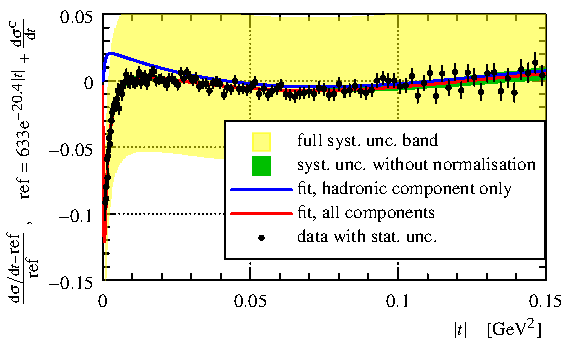
\includegraphics{fig/fit_details_exp3_0p15.pdf}
\caption{%
fit exp3, tmax 0.15,
\TODO{describe},
}
\label{fig:fit exp3 0.15}
\end{center}
\end{figure*}


\begin{figure*}
\vskip-5mm
\begin{center}
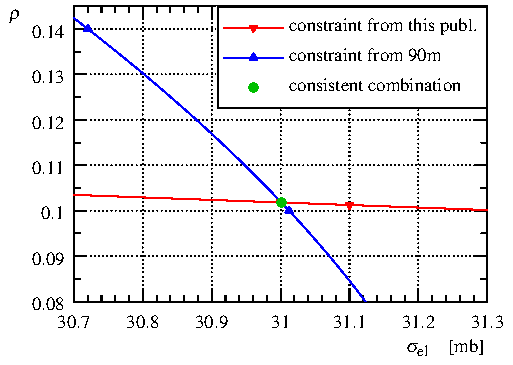
\includegraphics{fig/si_el_rho_solution.pdf}
\caption{%
\TODO{describe},
}
\label{fig:si_el rho sol}
\end{center}
\end{figure*}





\begin{figure*}
\vskip-5mm
\begin{center}
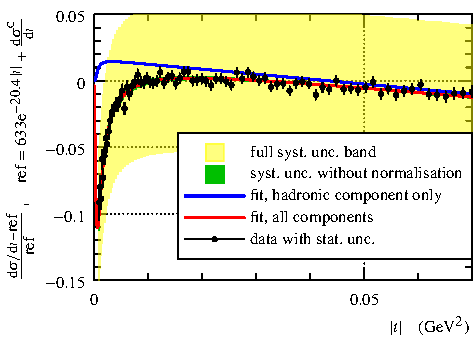
\includegraphics{fig/fit_details_exp1_0p07.pdf}
\caption{%
fit exp1, tmax 0.07,
\TODO{describe},
}
\label{fig:fit exp1 0.07}
\end{center}
\end{figure*}




\begin{figure*}
\vskip-5mm
\begin{center}
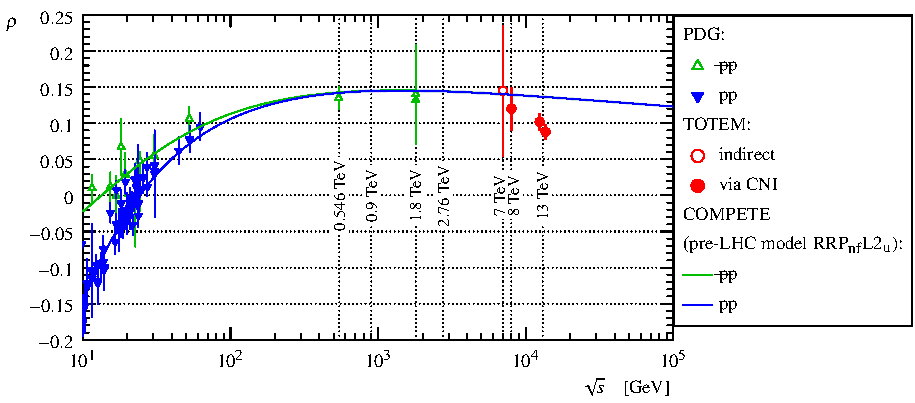
\includegraphics{fig/rho_vs_s.pdf}
\caption{%
\TODO{write}
}
\label{fig:rho_vs_s}
\end{center}
\end{figure*}
